\documentclass{article}
% --- watermark (auto-inserted) ---
\usepackage{xcolor}
\usepackage{xfp}% \fpeval; in the kernel since 2022, harmless on older LaTeX
\usepackage{draftwatermark}
\newlength{\watermarkTextWidth}
\AddToHook{begindocument/end}{%
  \SetWatermarkText{\normalfont Generated by The Agentic Scientist}%
  \SetWatermarkFontSize{10pt}%
  \SetWatermarkLightness{0.85}%
  \settowidth{\watermarkTextWidth}{\normalfont\fontsize{10pt}{12pt}\selectfont Generated by The Agentic Scientist}%
  \edef\watermarkScale{\fpeval{0.8 * sqrt(\paperwidth**2 + \paperheight**2) / \watermarkTextWidth}}%
  \edef\watermarkAngle{\fpeval{atand(\paperheight/\paperwidth)}}%
  \SetWatermarkScale{\watermarkScale}%
  \SetWatermarkAngle{\watermarkAngle}%
}
% --- end watermark ---

\usepackage{iclr2026_conference,times}
\usepackage{amsmath,amssymb,booktabs,graphicx,subcaption}
\usepackage{hyperref,url}
\newcommand{\clip}{\operatorname{clip}_{[0,1]}}
\newcommand{\MAE}{\operatorname{MAE}}
\title{Local Residual Transfer for Budgeted\\Embedding Benchmark Prediction}
\author{}

\begin{document}
\maketitle

\begin{abstract}
Predicting an embedding model's benchmark profile from a small evaluation budget requires both selecting informative benchmarks and transferring information from incomplete historical results. We study a low-rank predictor augmented with cross-fitted, locally weighted residual medians, evaluated on a pinned public MTEB score matrix. The predictor chooses queries by integrated variance reduction and calibrates residual transfer using historical models only. Across model and heuristic-family holdouts, three statistical seeds, and budgets of one, two, four, and eight queried task/subset columns, its aggregate mean absolute error is 0.04081, compared with 0.04525 for the strongest aggregate baseline. Error decreases from 0.04523 at one query to 0.03615 at eight. Historical-data disruptions delimit this finding: independent column shifts remove the advantage over column means. These results support the evaluated configuration on previously observed leaderboard cells, not causal attribution to residual transfer, prediction of genuinely missing results, or a universally sufficient evaluation budget.
% @evidence[[paper_data.json#/final_evaluation/metrics]]
% @evidence[[paper_data.json#/final_evaluation/evaluation_evidence/episodes]]
\end{abstract}

\section{Introduction}
Embedding evaluations measure different aspects of a representation, so a single score does not necessarily characterize performance on retrieval, semantic similarity, classification, and other uses. MTEB provides a public framework for evaluating this breadth \citep{MTEB}. Running a broad evaluation suite for every new model, however, is expensive. Historical score tables suggest a complementary approach: evaluate a new model on a small set of task columns and infer its remaining profile from relationships learned across previously evaluated models. This paper examines the statistical prediction problem, not the execution cost of the underlying benchmark workloads.

Two questions must be separated. Which columns should an evaluator measure under a fixed budget? And how should the resulting observations be converted into predictions? Low-rank structure offers a compact global description, but models with similar global representations may still share systematic residual errors. A local adjustment could exploit these similarities, while incomplete overlap and small donor neighborhoods could also make it unreliable. A useful study must therefore compare the complete predictor against meaningful alternatives, keep evaluation targets independent of the query policy, and test what happens when historical relationships are disrupted.

We investigate a concrete package: ridge-regularized alternating least squares (ALS), a greedy integrated-variance query policy, and a historical-only residual calibration procedure. For a new model, the residual adjustment uses historical donors that share queried columns, weights them by profile similarity and overlap, and transfers a shrunk weighted median of their held-out residuals. The design is deliberately conservative: historical validation can choose an exactly zero correction. We hypothesize that this package will lower absolute prediction error relative to simple means, low-rank references, and linear transfer in the observed-score regime. We do not hypothesize that the residual term alone causes any measured gain.

The evidence comes from one frozen embedding dataset, not a collection of unrelated leaderboards. Its final matrix contains 126 model rows and 135 task/subset columns. Under both model and heuristic-family holdouts, predictions are scored on a common sealed target set that remains unchanged as more queries are revealed. The aggregate MAE advantage over the strongest aggregate baseline is 0.00444 in normalized score units, or 9.82\% relative to that baseline. The same package loses its advantage over column means when historical column alignments are independently shifted. This boundary finding is part of the conclusion, rather than an exception to be excluded.
% @evidence[[source_evidence/resources/final/manifest.json]]
% @evidence[[derived_results.json#/relative_reduction]]
% @evidence[[paper_data.json#/final_evaluation/metrics/delta_best_baseline]]

Our contributions are a fully specified budgeted predictor, a fixed-target evaluation with dependence-aware paired uncertainty, and a measured failure boundary. Factorization, local weighting, and design have established antecedents; we do not claim novelty for these primitives or optimality of the complete configuration.

\begin{figure}[t]
\centering
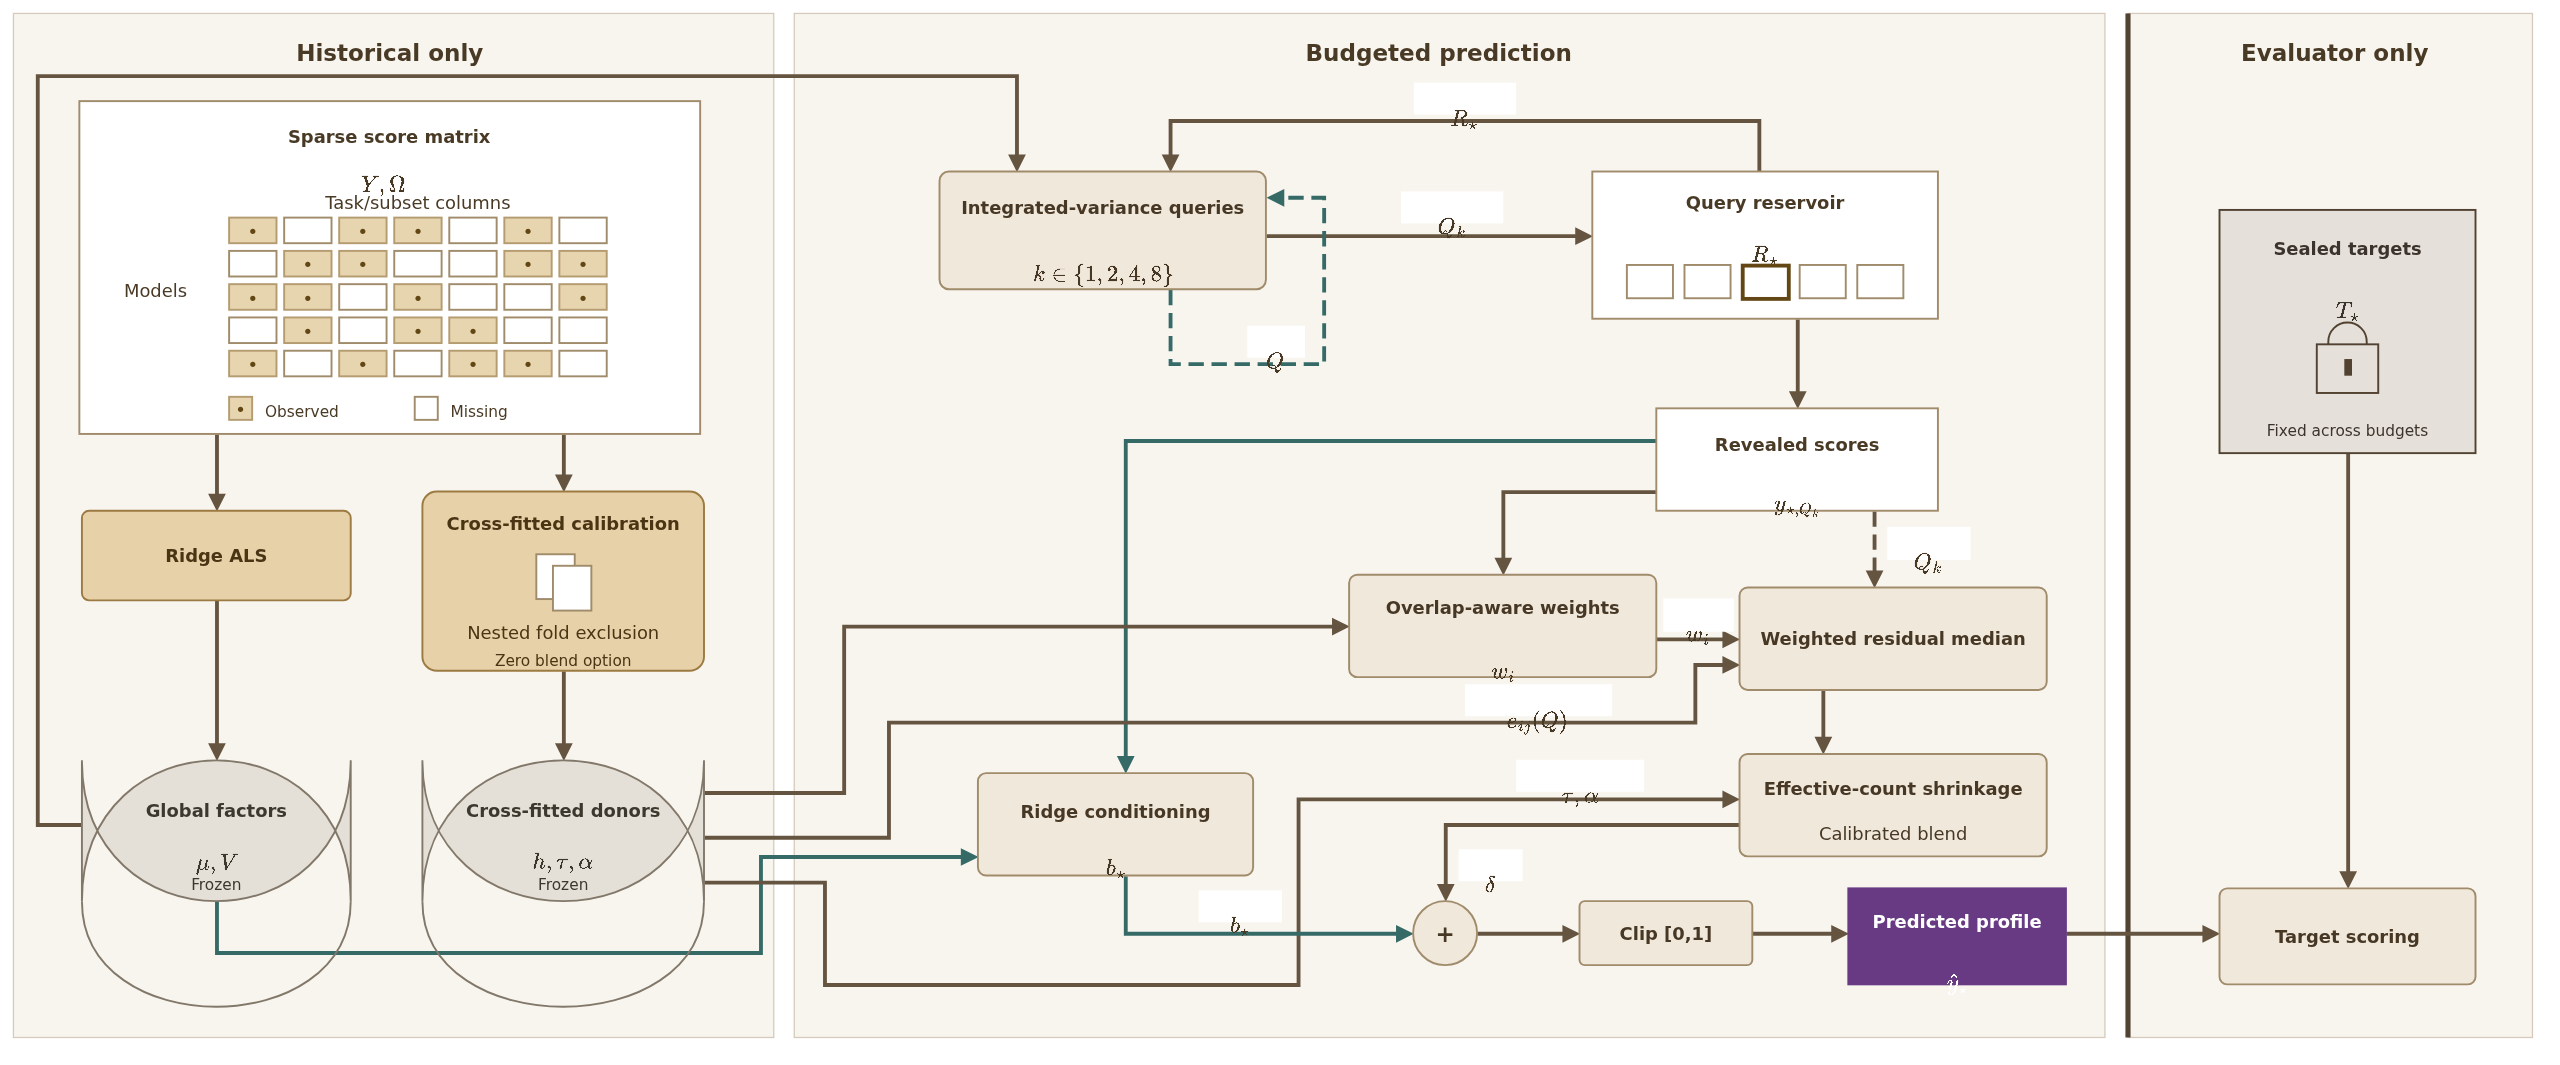
\includegraphics[width=\textwidth]{figures/method_overview.png}
\caption{Information boundaries of budgeted score prediction. Historical scores support global factor fitting and cross-fitted donor calibration. A held-out model supplies only queried scores; these condition its latent representation and local donor weights. Sealed evaluation targets are never passed to the predictor. Query indices depend on fitted factors and earlier indices, not on the revealed score values. The diagram describes the evaluated computation, not evidence of a component-specific benefit.}
\label{fig:overview}
% @evidence[[source_evidence/selected/src/program.py#L51-L315]]
% @evidence[[source_evidence/evaluate_final.py#L911-L967]]
\end{figure}

\section{Related Work}
\paragraph{Reducing evaluation and predicting performance.}
MTEB motivates studying broad embedding profiles rather than a single similarity task \citep{MTEB}. Neighboring work reduces evaluation at a different granularity: tinyBenchmarks selects small sets of examples, while metabench compresses reasoning and knowledge assessments into sparse item sets \citep{TinyBenchmarks,MetaBench}. Here the acquisition unit is an entire task/subset score, not an item response. Observational scaling laws and Sloth model performance through low-dimensional capabilities or skills across model families \citep{ObservationalScaling,Sloth}. They motivate compact cross-benchmark structure, but our experiment neither fits a compute-scaling law nor tests those approaches as baselines. In particular, evidence from generative-model evaluations cannot establish the present embedding predictor's accuracy.

\paragraph{Incomplete matrices and local prediction.}
Factor models and neighborhood methods are established tools for collaborative prediction \citep{Koren2009,Takacs2008}. Probabilistic and Bayesian factorization formalize latent-factor modeling and uncertainty over parameters \citep{Mnih2007,Salakhutdinov2008}; the present ALS estimator instead uses point estimates. Work on implicit feedback emphasizes observation semantics and confidence \citep{Hu2008}, whereas the present mask denotes an available benchmark score, not an implicit preference. Convex matrix completion, alternating minimization, and maximum-margin factorization supply distinct approaches to incomplete matrices \citep{Candes2009,Jain2013,Rennie2005}. Their recovery or optimization results are not guarantees for this selected leaderboard matrix. Local prediction has classical roots in neighbor classification and nonparametric regression \citep{Cover1967,Stone1977}; quantile regression connects medians with absolute-error objectives \citep{Koenker2001}. These connections motivate residual transfer without certifying its finite-sample behavior here.

\paragraph{Design and empirical inference.}
Bayesian experimental design and statistical active learning motivate selecting observations by expected information or prediction utility \citep{Chaloner1995,Cohn1996}. Ridge regularization stabilizes the small queried-column regression \citep{Hoerl1970}. Our covariance surrogate optimizes a linear variance criterion, not MAE itself. Missing-data theory cautions against interpreting observed-cell evaluation as recovery under arbitrary missingness \citep{Rubin1976}. Bootstrap reasoning motivates uncertainty assessment \citep{Efron1979}, but clustered dependence requires attention beyond treating rows or folds as independent \citep{Cameron2008,Bengio2004}. We retain the evaluator's component-paired construction and report its exact meaning rather than substituting seed-level error bars for inferential uncertainty.

\section{Method}
\subsection{Problem setup and design rationale}
Let $Y\in[0,1]^{M\times N}$ contain historical normalized scores and $\Omega$ their observed-entry mask. A new model has score vector $y_\star$, initially hidden. A query reservoir $R_\star$ specifies which indices can be acquired. Given a budget $k$, the predictor selects $Q_k\subseteq R_\star$, observes $y_{\star,Q_k}$, and returns an $N$-dimensional vector. The evaluation uses an evaluator-held target set $T_\star$ disjoint from the entire reservoir, not just from the selected indices. Its primary row loss is
\begin{equation}
 L_\star(k)=\frac{1}{|T_\star|}\sum_{j\in T_\star}|\widehat y_{\star j}(Q_k)-y_{\star j}|.
 \label{eq:loss}
\end{equation}
% @evidence[[source_evidence/evaluate_final.py#L851-L868]]
This target set is constant across methods and budgets. Therefore a lower loss cannot arise merely from querying and removing difficult target cells. The history contains no rows from the corresponding held-out partition, and new-model observations never update fitted historical state.

The design combines a global model with a conditional residual estimator. Global factors share information even when direct benchmark overlap is limited. Local donor profiles can represent deviations from the global fit, but missing anchors weaken neighborhood identification. We therefore use overlap-aware weights, donor-excluded predictions, effective-count shrinkage, and historical validation with a null correction. These are safeguards in the estimator, not evidence that all remaining bias or leakage is eliminated.

\subsection{Global fit and benchmark acquisition}
The historical mean $\mu_j$ is computed from observed entries in column $j$, with a neutral midpoint fallback if none is observed. Rank-$r$ row vectors $u_i$ and column vectors $v_j$ are fitted by alternating ridge solves for
\begin{equation}
 \min_{U,V}\sum_{(i,j)\in\Omega}(Y_{ij}-\mu_j-u_i^\top v_j)^2
       +\lambda\left(\sum_i\|u_i\|_2^2+\sum_j\|v_j\|_2^2\right).
 \label{eq:als}
\end{equation}
The evaluated settings are $r=4$, $\lambda=0.1$, and 50 sweeps; column factors start from independent zero-mean Gaussian entries with standard deviation 0.1. The historical means remain fixed. Only observed entries participate in the alternating solves; missing entries are not treated as observed zero scores.
% @evidence[[source_evidence/selected/src/program.py#L363-L388]]
% @evidence[[source_evidence/evaluate_final.py#L920-L939]]

For queried indices $Q$, define
\begin{equation}
 C_Q=(\lambda I+V_Q^\top V_Q)^{-1},\qquad
 z_\star=C_Q V_Q^\top(y_{\star,Q}-\mu_Q),\qquad
 b_\star=\clip(\mu+Vz_\star).
 \label{eq:condition}
\end{equation}
Here $V$ has row $v_j^\top$. For each unqueried reservoir index $a$, acquisition maximizes
\begin{equation}
 g(a\mid Q)=\frac{\sum_{j=1}^N(v_j^\top C_Qv_a)^2}{1+v_a^\top C_Qv_a}.
 \label{eq:query}
\end{equation}
% @evidence[[source_evidence/selected/src/program.py#L395-L426]]
This follows by substituting the rank-one update
$C_{Q\cup\{a\}}=C_Q-C_Qv_av_a^\top C_Q/(1+v_a^\top C_Qv_a)$
into the reduction of $\operatorname{tr}(VC_QV^\top)$. Thus the score is an exact reduction of this surrogate, with unit observation-noise convention, for the frozen factors. It is not a calibrated predictive posterior or a guarantee of lower realized absolute error. The sum includes \emph{all} columns, including the acquired column; it is not a target-only acquisition objective. The ordering depends on factors, the reservoir, and selected indices, so score feedback affects prediction but does not change subsequent index choices.

\subsection{Cross-fitted local residual transfer}
Historical donors are partitioned into folds. For each donor fold, an auxiliary factor model is fitted without those donors. A donor's available entries among $Q$ condition that model using Equation~\ref{eq:condition}; its finite observed target entries give residuals $e_{ij}(Q)=Y_{ij}-b^{(-i)}_{ij}(Q)$. The superscript denotes fold exclusion, not a separate fit for every donor. An unobserved donor target contributes no residual. Auxiliary predictions and the main base prediction are clipped before residual calculation or adjustment.
% @evidence[[source_evidence/selected/src/program.py#L97-L142]]

For donor $i$, let $A_i=Q\cap\Omega_i$ be its shared queried anchors and $s_{ia}$ the standard deviation of column $a$ in that donor's auxiliary fit, floored at 0.025. At bandwidth $h$, the profile distance and weight are
\begin{equation}
 d_i^2=\frac{\sum_{a\in A_i}[(Y_{ia}-y_{\star a})/s_{ia}]^2}{\max(|A_i|,1)},\qquad
 w_i=\frac{|A_i|}{|Q|}\exp[-d_i^2/(2h^2)].
 \label{eq:weights}
\end{equation}
Weights are zero without shared anchors. For column $j$, retain only donors with finite $e_{ij}$ and positive $w_i$, denoting this set $D_j$. Let $m_j=\operatorname{wmed}_{i\in D_j}(e_{ij};w_i)$ and compute
\begin{equation}
 n_j^{\mathrm{eff}}=\frac{(\sum_{i\in D_j}w_i)^2}{\max(\sum_{i\in D_j}w_i^2,10^{-12})},\quad
 \widehat y_{\star j}=\clip\left(b_{\star j}+\alpha\frac{n_j^{\mathrm{eff}}}{n_j^{\mathrm{eff}}+\tau}m_j\right).
 \label{eq:correction}
\end{equation}
% @evidence[[source_evidence/selected/src/program.py#L145-L197]]
The weighted median is the smallest sorted residual whose cumulative weight reaches half the total. It minimizes weighted absolute residual loss, but shrinkage and clipping need not preserve that minimizer. Total weight at most $10^{-12}$ leaves the base unchanged; the separate denominator floor in Equation~\ref{eq:correction} applies in prediction and calibration. Queried entries are not residual-adjusted. Without an active denominator floor, effective count measures weight concentration; when active, absolute weight scale also matters. Neither case certifies geometric support or extrapolation: equally weighted distant donors can still have a large count when the floor is inactive.

\subsection{Historical calibration and computational scope}
The correction is tuned without access to the held-out new model. Historical validation rows are split into two folds. Each validation fold is excluded from both its auxiliary base fit and its nested donor bank; donors are also excluded from the fits used to obtain their residuals. Querying is simulated within each historical validation row. Absolute errors are pooled over its finite unqueried cells at the same reporting budgets, then minimized over bandwidths $\{0.35,0.75,1.5\}$, shrinkages $\{4,16\}$, and blends $\{0,0.25,0.5,1\}$. Ties within the implemented tolerance favor the zero blend when it attains the minimum. The final donor bank is rebuilt from history after calibration.
% @evidence[[source_evidence/selected/src/program.py#L200-L297]]
This tuning target differs from the outer fixed-target loss: historical validation scores all available unqueried cells and pools cells, whereas the outer score averages row losses on sealed targets. The historical objective is a selection heuristic, not an unbiased estimate of the outer objective. There is no released outer comparison against the auxiliary unconditional-residual or direct-donor diagnostics computed during tuning.

Calibration caps the pool at $\min(512,\max(64,\lfloor196608/N\rfloor))$ rows, uses at most 128 donors and 16 validation rows, and limits auxiliary ALS to 12 sweeps. These are source-defined work limits, not measured runtime claims. For $E$ observed cells, one ALS sweep has dense-solve cost $O(Er^2+(M+N)r^3)$; auxiliary fits multiply this cost. Donor residual storage is bounded by donor count times column count, and query conditioning solves a small ridge system. These algebraic costs explain CPU feasibility at this matrix scale without establishing the storage or runtime of a full upstream leaderboard acquisition.
% @evidence[[source_evidence/selected/src/program.py#L200-L229]]

\section{Experimental Protocol}
\subsection{Data, normalization, and information access}
The public results snapshot is fixed to MTEB revision
\texttt{6dabbcc68c28ea5f180ce7df79347b3ca9cc6383}.
The retained final matrix has 126 rows and 135 columns, where a column identifies task, dataset revision, split, subset, and metric. These are not 135 independent benchmark suites. Extraction retains supported English text-only main metrics, checks their agreement with the reported main score, and chooses a common supported revision/metric/split per task/subset under the recorded coverage rule. Per-model revision selection favors coverage. Bounded noncorrelation scores remain in $[0,1]$; correlations are mapped by $(x+1)/2$. Hence errors are in normalized score units, not percentage-point errors uniformly comparable across raw metrics.
% @evidence[[source_evidence/resources/final/manifest.json]]
% @evidence[[source_evidence/evaluate_final.py#L685-L713]]

Canonicalized result content, row duplicates, aliases, and heuristic lexical-lineage families are used in partition construction. Model holdout excludes row, alias, and normalized-document overlap between history and test; family holdout additionally excludes the recorded family labels. The latter are heuristics, not verified model ancestry. Development and final partitions are also checked for the recorded identity, family, and content separation. Such checks reduce specified overlaps but cannot establish independence of training corpora or undocumented ancestry.
% @evidence[[source_evidence/evaluate_final.py#L715-L770]]

For each new-model row, the observed columns are shuffled deterministically and divided into a query reservoir containing approximately two thirds and a sealed remainder. The cut is at least eight columns, and each retained row has enough support for a nonempty target set. Targets and the complete target mask are withheld. The predictor receives an opaque indexed historical matrix, the queryable indices, and only the scores it requests. It cannot query genuinely missing cells in this experiment. Thus the study is a retrospective prediction test conditional on historical reporting, not evidence that unreported leaderboard scores can be recovered without selection bias.
% @evidence[[source_evidence/evaluate_final.py#L851-L863]]

\subsection{Comparators and matched controls}
The five references span simple, low-rank, and direct linear prediction. \emph{Column mean} returns the historical mean for each target. \emph{Query mean} assigns the new model's mean acquired score to every column. Both use variance-ranked queries where relevant. \emph{Random low-rank} and \emph{variance low-rank} fit the same rank and ridge family and condition on randomly ordered or historical-variance-ranked queries. \emph{Linear ridge} regresses centered target columns on the variance-ranked acquired columns, zero-filling missing centered historical entries in both its design and responses. Predictions are clipped where implemented. These low-rank references use different query policies from the studied package and therefore are not residual-only ablations.
% @evidence[[source_evidence/evaluate_final.py#L833-L902]]

Two controls reuse the model-holdout partitions and sealed targets. In the \emph{constant-history} condition every observed historical value is replaced by its column mean, preserving the mask. In the \emph{column-shifted} condition each column's values and masks are rolled together by an independently drawn nonzero row offset. This preserves the within-column observed-value multiset but perturbs cross-column alignment. Every method is refitted to the transformed history; the held-out model's answers are unchanged. These are data interventions on the full prediction system, not isolated interventions on residual transfer, and they do not guarantee removal of every dependence.
% @evidence[[source_evidence/evaluate_final.py#L808-L830]]

\subsection{Aggregation, uncertainty, and qualification}
Reporting budgets are $k\in\{1,2,4,8\}$, using nested query prefixes. Statistical seeds are 6841, 8089, and 9011. Most conditions use 94 historical and 32 test rows; the last family-holdout split uses 93 and 33. Within each condition and seed, losses average targets within a row, rows within a split, and the four budgets equally. The principal aggregate averages the two holdouts and three seeds equally. The strongest baseline is chosen by the minimum of these aggregate losses, not separately per row or budget. RMSE is the square root of the equally aggregated squared-error losses.
% @evidence[[source_evidence/resources/final/plan.json]]
% @evidence[[source_evidence/evaluate_final.py#L970-L996]]

For uncertainty, the evaluator draws 400 bootstrap multiplicity vectors over the union of recorded dependence components, with random seed 424242. A draw reweights the same component consistently wherever it appears across seeds and holdouts. Within each split, paired baseline-minus-studied row errors, averaged over budgets, are reweighted and normalized before equal split averaging. For each of five baselines, the 0.005 and 0.995 quantiles form the evaluator's Bonferroni-style bounds. The reported pair takes the minimum of the five lower bounds and separately the minimum of the five upper bounds. This is \emph{not} a conventional interval for a single prespecified comparator or the quantiles of a minimum-gain statistic. Finite bootstrap resolution, heuristic components, and shared data remain inferential limitations.
% @evidence[[source_evidence/evaluate_final.py#L999-L1017]]

The independent frozen evaluation completed and passed its qualification checks. Reset replay had identical query indices and maximum absolute prediction difference zero. These protocol checks do not certify universal validity or absence of every leakage source. Numerical displays use retained evaluator-owned losses, not unverified predictor diagnostics; no new model evaluation is performed for this paper.
% @evidence[[paper_data.json#/grounding_sources/final.qualification.status]]
% @evidence[[paper_data.json#/grounding_sources/final.qualification.outcome]]
% @evidence[[paper_data.json#/final_evaluation/metrics/reset_max_abs_delta]]

\section{Results}
\subsection{Main fixed-target comparison}
\begin{table}[t]
\centering
% @evidence[[paper_data.json#/final_evaluation/evaluation_evidence/episodes]]

\begin{tabular}{lrrr}
\toprule
Estimator & Model holdout & Family holdout & Overall \\
\midrule
Column mean & 0.06437 & 0.06411 & 0.06424 \\
Query mean & 0.23861 & 0.23562 & 0.23711 \\
Random low-rank & 0.04686 & 0.04933 & 0.04810 \\
Variance low-rank & 0.04479 & 0.04745 & 0.04612 \\
Linear ridge & 0.04512 & 0.04538 & 0.04525 \\
Residual transfer & 0.03831 & 0.04330 & 0.04081 \\
\bottomrule
\end{tabular}

\caption{Sealed-target MAE, lower is better, averaged equally over reporting budgets and seeds. Overall gives equal weight to model and heuristic-family holdouts. All five evaluated reference methods are included. Different acquisition policies prevent treating low-rank references as component ablations.}
\label{tab:main}
% @evidence[[paper_data.json#/final_evaluation/evaluation_evidence/episodes]]
\end{table}

The studied package attains aggregate MAE 0.04081 and RMSE 0.06432. Linear ridge is the strongest aggregate reference at MAE 0.04525, giving an absolute reduction of 0.00444 and relative reduction of 9.82\%. Table~\ref{tab:main} shows lower aggregate loss for the studied configuration than all five references in each holdout. This is a comparison between complete evaluated configurations. It does not identify which part of their fitting, acquisition, or prediction differences accounts for the reduction.
% @evidence[[paper_data.json#/final_evaluation/metrics]]
% @evidence[[derived_results.json#/primary_mean]]
% @evidence[[derived_results.json#/relative_reduction]]

The holdout distinction matters. The package's MAE is 0.03831 under model holdout and 0.04330 under heuristic-family holdout, whereas linear ridge gives 0.04512 and 0.04538. Removing recorded family overlap therefore coincides with a narrower advantage. Since these partitions also differ in their model composition, this contrast is not a controlled causal estimate of family membership or a demonstrated robustness guarantee for unseen true lineages.
% @evidence[[derived_results.json#/cases]]

The package's seed-level pooled MAEs are 0.03850, 0.04113, and 0.04280 (sample SD 0.00217), versus linear ridge's 0.04166, 0.04594, and 0.04815. These shared-data replications all favor the package. Component-bootstrap bound minima are $[0.00210,0.00920]$. Their positive lower minimum supports the aggregate comparisons under the specified construction; the endpoints need not correspond to the same baseline.
% @evidence[[derived_results.json#/primary_seed]]
% @evidence[[derived_results.json#/primary_seed_sd]]
% @evidence[[paper_data.json#/final_evaluation/metrics/gain_ci_low]]
% @evidence[[paper_data.json#/final_evaluation/metrics/gain_ci_high]]

\subsection{Accuracy versus query budget}
\begin{figure}[t]
\centering
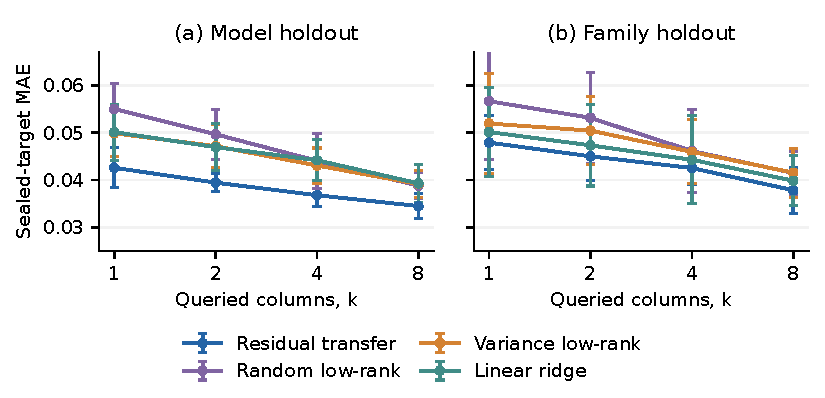
\includegraphics[width=\textwidth]{figures/budget_comparison.pdf}
\caption{Fixed-target MAE versus acquisition budget for model holdout (a) and heuristic-family holdout (b). Points average seeds; bars are descriptive sample standard deviations across the three seeds, not confidence intervals. Both panels share axes and retain the same targets across budgets. Simple references appear in Table~\ref{tab:main}; complete budget values are in the supplement.}
\label{fig:budget}
% @evidence[[paper_data.json#/final_evaluation/evaluation_evidence/episodes]]
\end{figure}

Across the two primary conditions, the package's MAEs at one, two, four, and eight queries are 0.04523, 0.04221, 0.03964, and 0.03615. Figure~\ref{fig:budget} separates the holdouts rather than masking their difference in a single curve. Their seed-averaged errors decrease at every reported budget; the same monotonicity is not asserted for every individual model. At eight queries, the package gives 0.03448 on model holdout and 0.03782 on family holdout, compared with linear ridge's 0.03927 and 0.03984.
% @evidence[[paper_data.json#/final_evaluation/metrics/mae_k1]]
% @evidence[[paper_data.json#/final_evaluation/metrics/mae_k2]]
% @evidence[[paper_data.json#/final_evaluation/metrics/mae_k4]]
% @evidence[[paper_data.json#/final_evaluation/metrics/mae_k8]]
% @evidence[[derived_results.json#/cases]]

More queried columns improve the reported aggregate over the tested range, but do not identify a universally adequate $k$. No application-specific tolerance or per-column execution costs were specified, and larger budgets were not measured. Moreover, the acquisition surrogate optimizes linear predictive variance, not sealed-target MAE.

\subsection{Dependence on historical structure}
\begin{figure}[t]
\centering
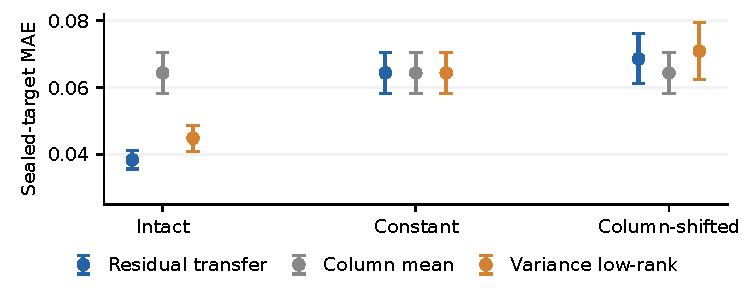
\includegraphics[width=.9\textwidth]{figures/history_structure_controls.pdf}
\caption{Matched model-holdout controls, averaged over budgets and seeds; bars show descriptive seed standard deviations. Constant history replaces each observed value by its historical column mean. Column-shifted history independently cyclically shifts each column's value/mask pairs. Small horizontal offsets separate overlapping points. The studied package does not beat column means after shifting; these conditions are not residual-only ablations.}
\label{fig:controls}
% @evidence[[paper_data.json#/final_evaluation/evaluation_evidence/episodes]]
\end{figure}

With intact history under model holdout, the package's MAE is 0.03831. Replacing historical observed values by column means raises it to 0.06437, equal to the column-mean and variance-low-rank references. Independently shifting columns yields MAE 0.06857, compared with 0.06437 for column means and 0.07091 for variance low-rank. Thus the package retains an advantage over the latter reference but is worse than the simpler historical mean in this disrupted condition. The appropriate intact comparator here is model holdout, not the pooled principal score.
% @evidence[[derived_results.json#/cases/A/mean]]
% @evidence[[derived_results.json#/cases/C/mean]]
% @evidence[[derived_results.json#/cases/D/mean]]

The constant condition is consistent with an estimator that falls back to column-level information when between-model variation vanishes. The shifted condition shows that preserving per-column value distributions is insufficient to retain the package's advantage. Neither observation identifies residual transfer as the cause: shifts change the factor fit, acquisition order, donor neighborhoods, and calibration simultaneously. Likewise, failure after disruption is not evidence that the intact-history result was invalid. It establishes a measured boundary under these particular matched transformations.

\section{Discussion and Limitations}
\paragraph{Prediction support and missingness.}
The conclusion concerns \emph{previously observed} scores in a frozen matrix. Reporting patterns can favor models and tasks with useful overlap, and availability may depend on performance or resources. The experiment neither identifies the missingness mechanism nor validates genuinely unreported-cell prediction. Normalization does not equalize application importance, and dependent task subsets are not independent scientific tests.

\paragraph{Attribution and estimator behavior.}
There is no matched outer comparison that removes only residual correction while preserving all other fitting and acquisition choices. Historical tuning diagnostics are not substitutes for such an ablation. The finite donor bank, short auxiliary fits, and limited shared anchors can induce residual estimation error; fold exclusion does not ensure residual unbiasedness. Effective-count shrinkage reflects concentration and, with an active denominator floor, absolute weight scale, but does not certify similarity. A history-chosen null blend cannot guarantee protection against a shifted new-model distribution. The observed control failure qualifies the predictor's usefulness without establishing a mechanism.

\paragraph{Generalization and uncertainty.}
Family separation is based on lexical-lineage heuristics and duplicate closure, not exhaustive knowledge of shared pretraining or adaptation. There is only one pinned leaderboard and no temporal, cross-leaderboard, or generative-model evaluation. Bootstrap bounds are conditional on recorded components, with a finite number of draws and shared source data. Their positive lower minimum is evidence within this construction, not an unconditional statistical guarantee. Architectural or missingness-stratified generalization and calibrated predictive intervals remain unmeasured.

\paragraph{Selection and practical use.}
The evaluated configuration was frozen after development comparisons, so those comparisons are not independent confirmation or controlled component tests. A separate support-gating variant did not yield a retained numeric performance result; its failure cause is not diagnosed and cannot be counted as a measured loss. The final qualification passed, but this does not erase selection uncertainty or the limitations above. For deployment, the appropriate fallback depends on uncertainty about historical comparability, not only the intact-matrix aggregate. The current evidence motivates testing such decisions; it does not validate a switching rule or establish end-to-end savings.
% @evidence[[paper_data.json#/all_programs]]
% @evidence[[paper_data.json#/grounding_sources/final.qualification.outcome]]

\section{Conclusion}
Budgeted embedding evaluation can be studied as prediction from an incomplete historical score matrix with controlled access to a held-out model. In the retained MTEB evaluation, a low-rank predictor with historically calibrated local residual transfer has lower aggregate sealed-target MAE than the five evaluated references, and its aggregate error decreases over the tested budgets. Fixed targets make these differences interpretable without letting acquisition remove difficult evaluation cells, while component-paired resampling preserves some important dependencies.

Disrupting historical column alignment removes the advantage over column means, and the comparisons do not isolate a residual-specific causal effect. Observed-cell prediction with heuristic family separation does not establish recovery of genuinely missing scores, transfer to generative models, or a generally sufficient budget. The finding is a configuration-level advantage with an explicit failure boundary: historical score structure can support compact evaluation, but its suitability must be examined rather than assumed.

\clearpage
\bibliography{references}
\bibliographystyle{iclr2026_conference}

\clearpage
\appendix
\begingroup
\renewcommand{\thesection}{}
\section{Supplementary Information}
\endgroup
\thispagestyle{plain}
\subsection{Observed-score extraction and split provenance}
The final data manifest records selection of a modal supported dataset revision, split, and metric per task/subset with at least 32 rows globally, followed by a maximal-coverage model revision and a minimum of 12 cells per retained row. Normalized task/version/score content is canonicalized using Unicode normalization, whitespace normalization, sorted keys, and integral-number canonicalization while excluding source identifiers and timing. The recorded allocation uses family lexical-lineage heuristics and document/row duplicate closure, then assigns components to disjoint development and final partitions. The final evaluator re-extracts scores from retained source documents and checks content integrity, alias overlap, and split constraints. These checks are inspectable in the accompanying source; the fingerprints alone do not substantiate extraction semantics.
% @evidence[[source_evidence/resources/final/manifest.json]]
% @evidence[[source_evidence/evaluate_final.py#L666-L770]]

Task definitions are pinned to metadata repository revision
\texttt{5a83aafe4e7140d0606b96f59448c704f31dbf76}.
The manifest records CC0-1.0 evidence for results and Apache-2.0 for metadata, but also records that the results license was absent from the pinned results snapshot. Thus the available current-license evidence should not be represented as an unambiguous historical license grant at that snapshot. Public access and the presence of a repository license do not resolve all underlying benchmark-data terms. The bundled source documents and their hashes permit checking the matrix without downloading repository history; upstream acquisition should use the exact revision recorded in the manifest.
% @evidence[[source_evidence/resources/final/manifest.json#/license_evidence]]

\subsection{Residual calibration specification}
\begin{table}[h]
\centering
\begin{tabular}{ll}
\toprule
Setting & Evaluated value or source-defined cap \\
\midrule
Main ALS & Rank 4; ridge 0.1; 50 sweeps \\
Auxiliary ALS & At most 12 sweeps \\
Historical validation & At most 16 rows; two validation folds \\
Donor construction & At most 128 donors; two donor folds \\
Bandwidth & $0.35,\ 0.75,\ 1.5$ \\
Shrinkage & $4,\ 16$ \\
Blend & $0,\ 0.25,\ 0.5,\ 1$ \\
Distance scale floor & $0.025$ \\
Negligible total weight & $10^{-12}$ \\
\bottomrule
\end{tabular}
\caption{Implementation settings, not empirically isolated optimal choices. Historical pool size is capped by the expression in the main text.}
\label{tab:settings}
% @evidence[[source_evidence/selected/src/program.py#L51-L297]]
% @evidence[[source_evidence/evaluate_final.py#L920-L939]]
\end{table}

For each validation fold, remove its rows from the historical fitting pool. Fit the auxiliary base on the remaining rows, select a donor pool from those rows, and split donors into two folds. For each donor fold, fit without that fold, retaining only observed donor scores. For a validation row, simulate the same acquisition criterion on its available scores. Cache donor-excluded predictions for each queried index tuple; the cache affects computation but not access to targets. At each reporting budget, evaluate the clipped base plus each candidate correction on finite unqueried validation cells. Pool absolute-error sums and target counts across these cells and folds, select bandwidth/shrinkage/blend, and rebuild the donor bank from historical data. If support checks fail, retain the zero-blend configuration. Auxiliary randomness uses a separate seed sequence, preserving the main-fit random stream.
% @evidence[[source_evidence/selected/src/program.py#L110-L297]]

The code also calculates unconditional residual and direct donor-score diagnostics during this process. No outer results for those choices are retained. Neither their existence nor historical selection of a nonzero correction demonstrates an outer improvement relative to a fully matched zero-correction configuration. The main estimator's clipped base and donor-specific auxiliary bases are not identical fitted models, so fold exclusion should not be interpreted as an exact decomposition of outer prediction error.

\subsection{Complete primary comparisons}
\begin{table}[h]
\centering
\small
% @evidence[[paper_data.json#/final_evaluation/evaluation_evidence/episodes]]

\begin{tabular}{llrrrr}
\toprule
Holdout & Estimator & $k=1$ & $k=2$ & $k=4$ & $k=8$ \\
\midrule
Model & Column mean & 0.06437 & 0.06437 & 0.06437 & 0.06437 \\
Model & Query mean & 0.25893 & 0.24443 & 0.23056 & 0.22051 \\
Model & Random low-rank & 0.05498 & 0.04965 & 0.04403 & 0.03877 \\
Model & Variance low-rank & 0.04986 & 0.04713 & 0.04305 & 0.03914 \\
Model & Linear ridge & 0.05010 & 0.04694 & 0.04416 & 0.03927 \\
Model & Residual transfer & 0.04258 & 0.03943 & 0.03677 & 0.03448 \\
\midrule
Family & Column mean & 0.06411 & 0.06411 & 0.06411 & 0.06411 \\
Family & Query mean & 0.25572 & 0.23810 & 0.23156 & 0.21710 \\
Family & Random low-rank & 0.05664 & 0.05312 & 0.04611 & 0.04146 \\
Family & Variance low-rank & 0.05192 & 0.05042 & 0.04594 & 0.04152 \\
Family & Linear ridge & 0.05012 & 0.04731 & 0.04426 & 0.03984 \\
Family & Residual transfer & 0.04789 & 0.04499 & 0.04251 & 0.03782 \\
\bottomrule
\end{tabular}
\caption{Complete seed-averaged sealed-target MAE by holdout and budget. Low-rank is abbreviated LR in the seed table. All values derive from the same retained row/checkpoint arrays.}
\end{table}
\begin{table}[h]
\centering
\small
% @evidence[[paper_data.json#/final_evaluation/evaluation_evidence/episodes]]

\begin{tabular}{lrrrrrr}
\toprule
Seed & Col. mean & Query mean & Random LR & Var. LR & Ridge & Studied \\
\midrule
6841 & 0.05946 & 0.23783 & 0.04536 & 0.04282 & 0.04166 & 0.03850 \\
8089 & 0.06262 & 0.23947 & 0.04751 & 0.04596 & 0.04594 & 0.04113 \\
9011 & 0.07063 & 0.23404 & 0.05142 & 0.04959 & 0.04815 & 0.04280 \\
\midrule
Seed SD & 0.00575 & 0.00278 & 0.00307 & 0.00339 & 0.00330 & 0.00217 \\
\bottomrule
\end{tabular}
\caption{Sealed-target MAE averaged equally over primary holdouts and budgets within each seed; SD is descriptive sample standard deviation. Shared source data preclude interpreting these as independent dataset replications.}
\end{table}

The baseline-specific component-bootstrap bounds, in the order column mean, query mean, random low-rank, variance low-rank, and linear ridge, are respectively $[0.01538,0.04037]$, $[0.18530,0.20768]$, $[0.00412,0.01426]$, $[0.00340,0.00920]$, and $[0.00210,0.00939]$. They bound baseline-minus-studied errors under the retained construction. Taking lower and upper minima separately produces the reported pair; it does not select a single baseline interval. The evaluator's zero-weight-split convention inserts a conservative negative gain for such a bootstrap split. The reproduction script preserves that convention rather than silently dropping the split.
% @evidence[[derived_results.json#/baseline_gain_bounds]]
% @evidence[[source_evidence/evaluate_final.py#L999-L1017]]

\subsection{Changing-target diagnostic and disruption interpretation}
The evaluator also records loss over all observed but currently unqueried cells. Seed- and budget-averaged values for the studied package are 0.03665 on model holdout, 0.04242 on family holdout, 0.06528 with constant history, and 0.06352 with shifted history. This diagnostic changes its evaluated cell set as acquisitions accumulate and can also differ across query policies. It is therefore not used for the principal comparative claim. In particular, its shifted-history value cannot be substituted for the sealed-target control result.
% @evidence[[derived_results.json#/changing_target_mae]]

In the constant control, all methods using only centered historical linear variation collapse to the same column means on sealed targets in the retained arrays. The query-mean reference remains different because it uses real new-model query values rather than the collapsed historical values. Column shifting preserves each column's observed scores and count, including the value/mask pairing, but not the row-wise alignment. These controls distinguish information in per-column distributions from information in cross-column relationships at the package level; they do not isolate a correction mechanism or prove that every relationship has been destroyed.
% @evidence[[derived_results.json#/cases/C/mean]]
% @evidence[[source_evidence/evaluate_final.py#L808-L830]]

\subsection{Reproducibility and incomplete evidence}
The accompanying \texttt{README.md} maps source files, commands, dependencies, and data versions. Readable snapshots preserve the evaluated estimator, the original predictor, and the final evaluator. Figures and numeric tables are generated by \texttt{build\_paper\_artifacts.py} from the immutable evidence registry, using NumPy for array computations and Matplotlib for quantitative plots \citep{Harris2020,Hunter2007}. The conceptual overview is a qualitative diagram with separate rendering provenance. No schematic numeric values are used as experimental results. Every quantitative display has an input trail; source locations support implementation claims separately from file fingerprints.

Development selection was adaptive and preceded freezing the final configuration. Two development configurations had numeric scores; a support-gating configuration had no retained numeric score after evaluation failure. The failure diagnostics do not identify whether that failure was statistical, implementation-related, or due to another condition. It is missing performance evidence, not a measured loss, and neither development comparison is a matched final ablation. This paper uses the independent final evaluation for its quantitative comparisons. No additional ablation, temporal holdout, missingness stratification, or cross-leaderboard study was completed for the manuscript.
% @evidence[[paper_data.json#/all_programs]]
% @evidence[[paper_data.json#/grounding_sources/result.total_evaluated_programs]]

Retrieved reference metadata and consulted abstracts are retained locally with provenance links. The literature discussion is limited to that consulted content and does not claim an exhaustive search or establish priority.

\subsection{LLM Usage}
Language models assisted with research hypothesis formulation, implementation drafting, reference-query planning, manuscript framing, writing, and evidence/validation code. The paper-writing assistant inspected the retained implementation and evaluator, generated deterministic summaries and plots from retained arrays, and revised the manuscript against compilation and grounding checks. The numerical model-evaluation evidence comes from the frozen evaluator, not language-model-generated measurements. Language-model assistance does not provide independent verification of novelty or statistical validity. The conceptual-figure workflow may use model-assisted rendering; this does not introduce additional empirical evidence.

\end{document}
